% A simple example showing how to create Harvard-style referencing in LaTeX
% 
% See http://tex.stackexchange.com/questions/102662/harvard-reference-using-biblatex
% for further discussion
\documentclass[12pt]{article}

\usepackage[english]{babel}
\usepackage[utf8]{inputenc}
\usepackage{amsmath}
\usepackage{csquotes}% Recommended
\usepackage{geometry}
% \usepackage{url}
\usepackage{graphicx}
\usepackage{hyperref}
\usepackage{float}
\usepackage[font=small]{caption}
\captionsetup{justification=centering}
\hypersetup{
    colorlinks=true,
    citecolor = magenta,
    urlcolor=blue,
    % pdftitle={Overleaf Example},
    % pdfpagemode=FullScreen,
}

\urlstyle{same}

\geometry{top=50pt}
\usepackage[style=authoryear-ibid,backend=biber]{biblatex}

\addbibresource{sample.bib}% Syntax for version >= 1.2

\title{Should scientists and bioengineers be able to use CRISPR for germline editing?}
\author{Harsh Agrawal, Iva-Mari Miškulin, \\ Jiayi Bai, Piotr Skubis, Povilas Sauciuvienas}
\date{}

\begin{document}
\maketitle
\subsection*{Introduction}
The advances in genetic engineering and CRISPR-Cas9 technology have resulted in
an unprecedented ethical dilemma: humanity has gained the tools required to
edit the genomes of unborn children before considering whether they should be
employed. Germline editing holds the potential to not only eliminate grave
genetic disorders, such as sickle cell anemia or Huntington's disease before a
child is born, but also to eventually prevent illnesses (e.g., by increasing
resistance to cancer or contagious diseases) \parencite{gyngell_2017}.

However, our limited understanding of gene function and interplay poses a risk
of unintended complications and threatens the treated child's health and
well-being \parencite{frosch_2022}. Moreover, germline editing could be misused
for objectives akin to eugenics: regulating intelligence, eye color, and other
mental or physical attributes \parencite{sufian_2021}. Even though germline
editing is outlawed in most western countries \parencite{araki_ishii_2014}, the
unparalleled abilities it promises cannot be refuted \parencite{gyngell_2017};
thus it is necessary to discuss to what extent germ cell editing should play a
role in our society.

\subsection*{Course of Action}
Currently, germline editing is universally prohibited; however, it is not the
only possible course of action for the future. As our experience with genetic
engineering advances, we might reach a point where germline editing can offer
cures for select illnesses where no other solutions are currently available.
While still viewed as ethically undesirable for widespread use, gene editing
might be employed as a last resort.

Furthermore, germline editing has the potential to become a standard medical
procedure. Susceptibility to genetic disorders could be screened in couples who
plan to conceive, and the results could be used as a recommendation for genetic
engineering.

Another, although unlikely, possibility is germline editing being fully
embraced by society. This would give individuals full power and the ability to
decide how to apply germline engineering.

\subsection*{Discussion}

Currently, the majority of western nations have either banned or discouraged
research on germline editing due to ethical concerns
\parencite{araki_ishii_2014}. In December 2015, an international effort led by
the UK, USA, and China was launched during the International Summit on Gene
Editing with the aim of preventing and prohibiting germline editing. It was
also found that highly religious groups are more likely to oppose the idea of
germline editing \parencite{funk_kennedy_sciupac_2020}. Apart from just being
an ethical dilemma, germline editing threatens to exacerbate existing
prejudices and wealth-based inequalities \parencite{cbs_news_2021}. Moreover,
it can have unforeseen long-term consequences, such as the emergence of novel
pathogenic genes and/or the elimination of unknown positive effects of the
modified genes \parencite{rubeis_steger_2018}. One of the primary concerns
regarding germline editing is its use for eugenics, such as modifications made
to optimize appearance and intelligence
\parencite{world_health_organization_2021}.

However, it cannot be ignored that this technology can be employed to treat
forms of genetic infertility and prevent grave inherited diseases, which would
allow individuals to conceive healthy children \parencite{rubeis_steger_2018}.
Since a significant portion of inheritable diseases do not have an approved
treatment \parencite{department_uk_2021}, germline engineering might be the
only way to improve quality of life. If germline editing is to be employed only
in certain cases, deciding which conditions are `grave enough' to warrant the
risk of complications is key, considering our current limited understanding of
gene interplay \parencite{rubeis_steger_2018}.

As the safety and adoption of genetic engineering grow, this technology can be
embraced for a broader societal benefit. Germline editing could become a
standard medical procedure in treating conventional diseases, such as
hypertrophic cardiomyopathy \parencite{ledford_2017}. There is even a
possibility of eradicating entire genetic diseases from our population in a
humane way. Furthermore, one should consider if parents have the right to
choose who they want their children to be and how they look, as do individuals
really have free will if everything has been predetermined by one's parents. In
the case of CRISPR and designer babies, this free will would be intruded upon.
The arguments presented demonstrate the difficulty in choosing a prudent course
of action from the ones outlined above, which only exemplifies the need for
further discussion if we wish to reap the benefits of this technology.

\begin{figure}[H]
    \centering
    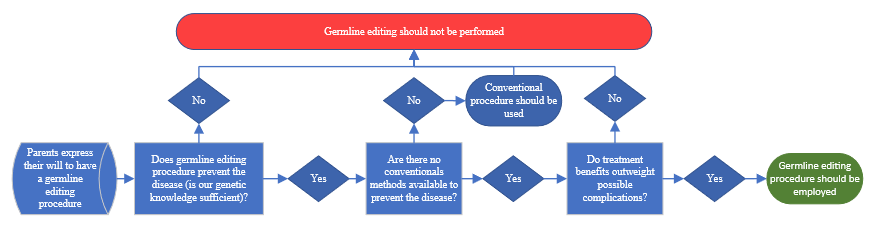
\includegraphics[width=0.8\textwidth]{flowchart.png}
    \caption{The following represents our decision tree on when germline editing be allowed to prevent grave diseases}\label{fig:my_label}
\end{figure}

\printbibliography[]

\end{document}